\chapter{Probe Training, Calibration, and Cross-Domain Transfer}
\label{ch:probe_training}

Having described the architecture, we now turn to how the probes are actually trained, how we ensure their outputs are well-calibrated, and critically whether the learned signals hold up when tested on data the probes have never seen before.

%% -------------------------------------------------
\section{Probe Architecture and Training Protocol}
\label{sec:training_protocol}

For each backbone, we train two independent MLP probes: one that receives the CEV feature vector $\boldsymbol{\phi}(\mathbf{x})$, and another that receives the IAV feature vector $\boldsymbol{\psi}(\mathbf{x})$. Both use the same two-hidden-layer architecture described in Section~\ref{sec:probe_arch} (Table~\ref{tab:probe_architecture}), but they accept different input dimensions since CEV and IAV come from different representational spaces.

The label convention is straightforward: $y = 0$ means the response is grounded (supported by the retrieved context), and $y = 1$ means it is hallucinated. After training converges, we apply temperature scaling to turn the raw logits into calibrated probabilities—a step that matters a great deal when the downstream controller makes decisions based on absolute probability values rather than just rankings.

Table~\ref{tab:training_config} consolidates the full training recipe.

\begin{table}[!htb]
\centering
\caption{Probe training configuration.}
\label{tab:training_config}
\begin{tabular}{@{}ll@{}}
\toprule
\textbf{Parameter} & \textbf{Setting} \\
\midrule
Probe type              & Two independent MLP probes: CEV and IAV \\
Optimizer               & AdamW \\
Learning rate           & Mistral: $3 \times 10^{-4}$;\; LLaMA/Qwen: $1 \times 10^{-3}$ \\
Scheduler               & CosineAnnealingLR \\
Minimum learning rate   & $1 \times 10^{-6}$ \\
Loss function           & Class-weighted cross-entropy \\
Label smoothing         & $\varepsilon = 0.05$ \\
Maximum epochs          & 40 \\
Early stopping criterion & Validation AUROC \\
Early-stopping patience & 10 epochs \\
Validation split        & Stratified 80/20 from RAGTruth training data \\
Checkpoint selection    & Best validation AUROC \\
\bottomrule
\end{tabular}
\end{table}

Why these specific choices? The class weighting corrects for label imbalance, the label smoothing prevents overconfident predictions (which would hurt calibration), and the per-backbone learning rates reflect empirical tuning Mistral's activations turned out to be more format-sensitive and needed a gentler optimizer step. The full rationale is in Section~\ref{sec:probe_training_details}.

%% -------------------------------------------------
\section{Training Dynamics and HaluEval Transfer}
\label{sec:training_dynamics}

Figure~\ref{fig:training_halueval} tells two stories at once. The top row shows how training progresses on the RAGTruth validation split, our in-domain sanity check. The bottom row asks a harder question: do these probes still work when applied to HaluEval, a completely different hallucination benchmark they were never trained on?

\begin{figure}[!htb]
    \centering
    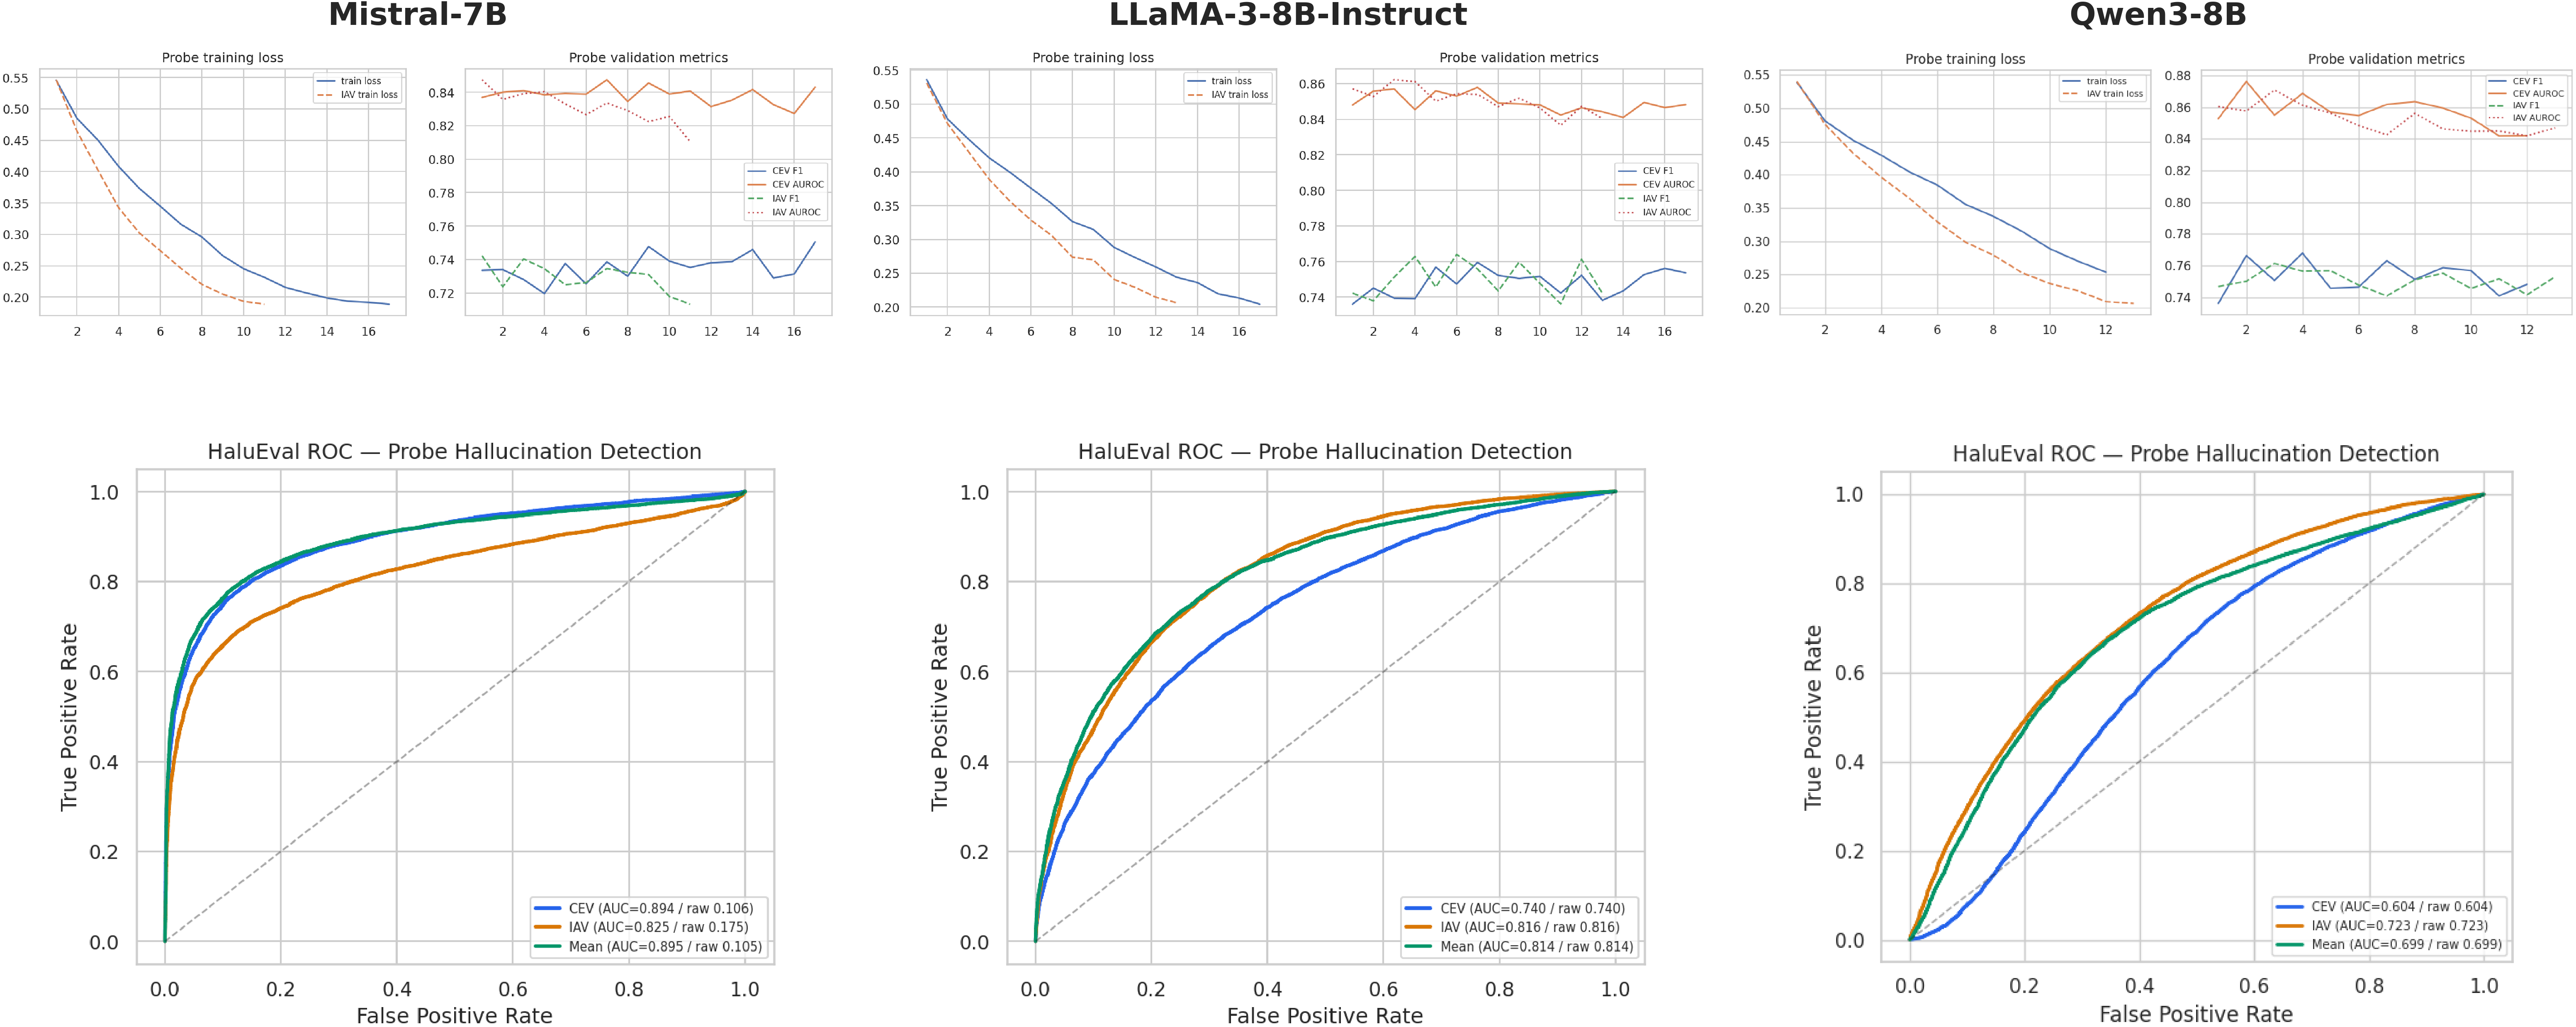
\includegraphics[width=1.05\textwidth]{Images/compare_training_and_halueval_grid.png}
    \caption[Probe training dynamics and HaluEval cross-domain ROC curves.]{Top row: in-domain training loss and validation AUROC for all three backbones. Bottom row: HaluEval out-of-domain ROC curves for CEV, IAV, and fused scores.}
    \label{fig:training_halueval}
\end{figure}

\newpage
\subsection{In-Domain Training Behavior}
\label{sec:indomain_training}

The good news first: training is well-behaved across the board. Loss curves decrease smoothly for both CEV and IAV probes on all three backbones—no instability, no sudden collapses. Validation AUROC climbs and then plateaus, which tells us the probes are learning genuine patterns rather than memorizing training examples.

What is particularly encouraging is that the dual-signal design holds up empirically. IAV tends to be the stronger individual branch, but CEV is never far behind and clearly contributes complementary information. This validates our choice to train two separate probes and fuse them, rather than betting everything on a single signal source.

\subsection{HaluEval Cross-Domain Transfer}
\label{sec:halueval_transfer}

The bottom row of Figure~\ref{fig:training_halueval} is where things get interesting—and, for one backbone, surprising.

For LLaMA-3-8B-Instruct and Qwen3-8B, transfer works as one would hope. The raw AUROC values land above 0.5, meaning the probes trained on RAGTruth still assign higher hallucination scores to the hallucinated HaluEval answers than to the correct ones. The signal generalizes.

Mistral-7B-Instruct-v0.2 is a different story. Its raw AUROC values are far \emph{below} 0.5 around 0.105. At first glance this looks like a catastrophic failure. But look more carefully: an AUROC of 0.105 is not random (which would give 0.5). It means the probe is separating the classes \emph{very well} just in the opposite direction. The adjusted value of $1 - 0.105 = 0.895$ tells us the discriminative power is actually excellent; the polarity just flipped under distribution shift.

The full numerical breakdown is in Table~\ref{tab:halueval_ood} (Section~\ref{sec:halueval_ood}). We do not repeat the numbers here.

\subsection{Interpretation of Mistral Polarity Inversion}
\label{sec:polarity_inversion}

This polarity inversion deserves careful interpretation. It is \emph{not} a bug in the code, if it were random noise, the AUROC would hover around 0.5, not plunge to 0.105. And it is not caused by using a base model instead of an instruction-tuned one; we explicitly use the fully tuned Mistral-7B-Instruct-v0.2 checkpoint.

What seems to be happening is that Mistral's internal representations encode hallucination-relevant information in a way that is directionally specific to the training distribution. When the distribution shifts (from RAGTruth to HaluEval), the \emph{meaning} of certain activation patterns flips. The signal is strong but its sign reverses.

The practical takeaway is sobering but important: \emph{you cannot assume that an internal-state probe will transfer automatically to a new domain, benchmark, or prompt format.} Before deploying in a new setting, the probe needs to be validated and possibly recalibrated on representative examples from the target distribution.

\subsection{Comparison with the Triple-Layer Configuration}
\label{sec:triple_comparison}

One might wonder whether the three-layer concatenation handles distribution shift better than our single mid-layer approach; maybe the extra depth diversity helps with generalization? We checked. It does not.

\begin{figure}[!htb]
    \centering
    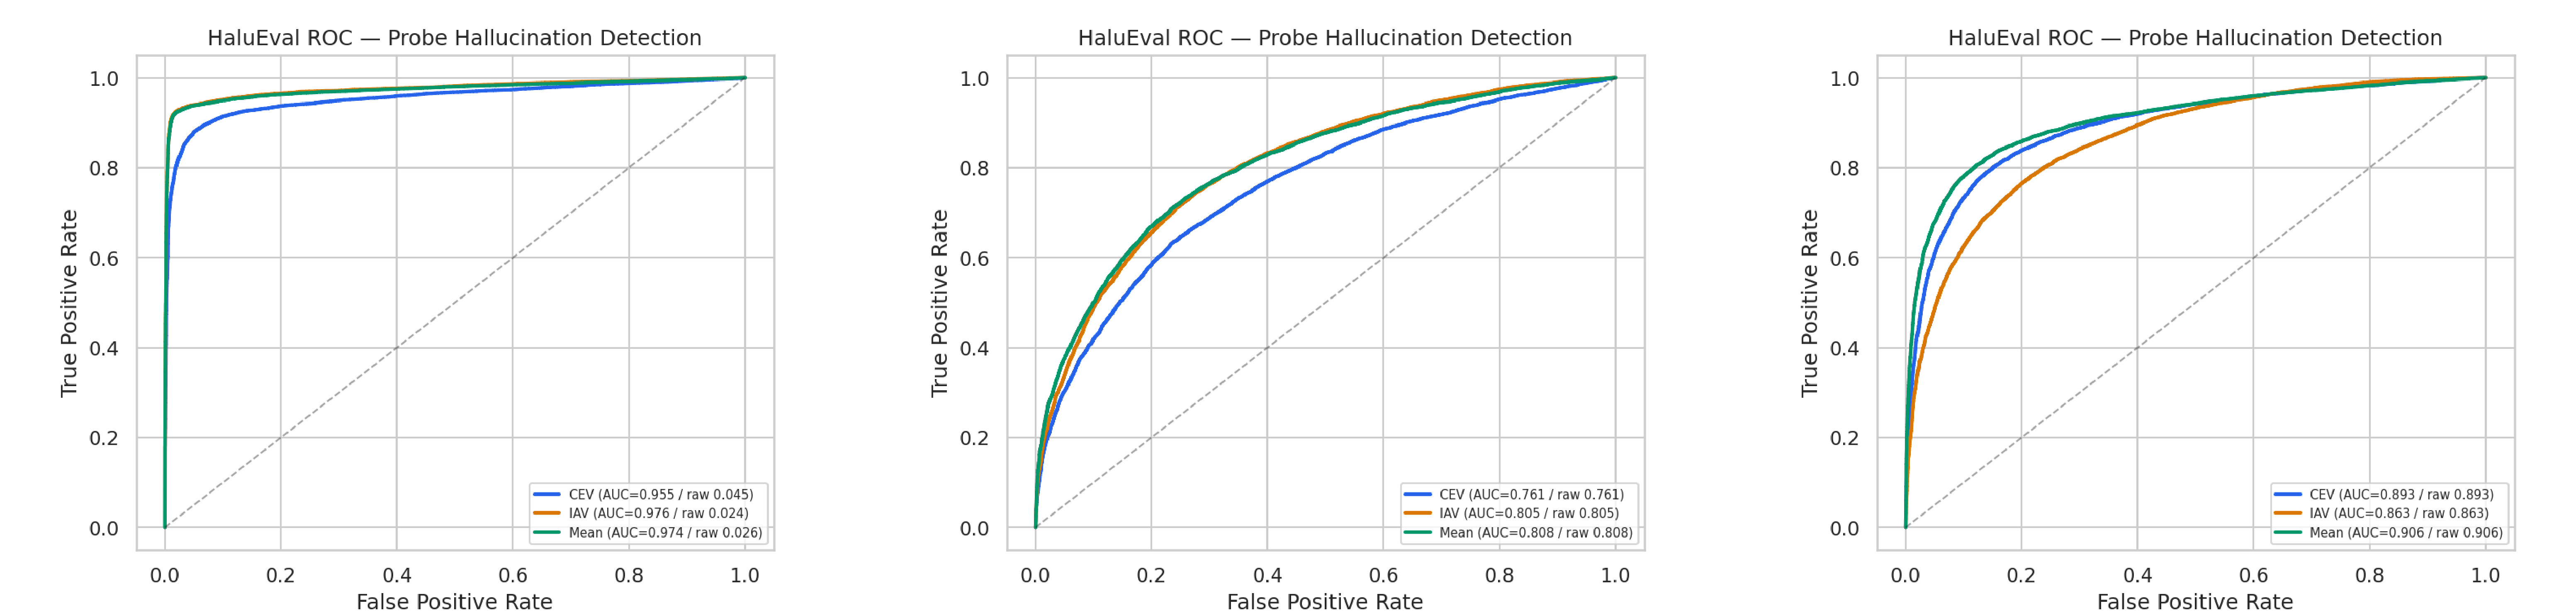
\includegraphics[width=1.00\textwidth]{Images/triple_compare_training_and_halueval_grid.png
}
    \caption[Triple layer Probe training dynamics and HaluEval cross-domain ROC curves.]{Per-backbone HaluEval ROC  for the three-depth (triple) concatenation. }
    \label{fig:Triple layer training_halueval}
\end{figure}



The triple configuration produces nearly identical training curves and HaluEval ROC behavior. Mistral still shows polarity inversion. LLaMA and Qwen still show aligned transfer. No metric meaningfully improves over the single mid-depth result. The extra parameters buy nothing, which further validates the layer-selection decision from Section~\ref{sec:layer_selection}.

%% -------------------------------------------------
\newpage
\section{Post-Training Calibration and Fusion}
\label{sec:calibration_fusion}

Once training is complete, we calibrate each probe independently using temperature scaling:
\begin{equation}
    P(y = 1) = \text{softmax}\!\left(\frac{\mathbf{z}}{T}\right)
\end{equation}

\noindent The temperature $T$ is found by minimizing validation negative log-likelihood. Why bother with this step? Because the controller makes threshold-based decisions. If the probe outputs 0.65 when it really means 0.45, the controller will over-intervene. Calibration ensures that the probability values \emph{mean what they say}.

We calibrate CEV and IAV separately because the two probes can have quite different confidence profiles. One might be well-ranked but systematically overconfident; the other might be better calibrated but with weaker discrimination. Temperature scaling brings them onto a common scale before fusion.

After calibration, the two probabilities are combined:
\[
    p_{\text{fused}} = w \cdot p_{\text{CEV}} + (1 - w) \cdot p_{\text{IAV}}
\]

\noindent with $w$ selected by grid search on the validation split to maximize AUROC. Importantly, this fusion happens at the \emph{probability} level—not by concatenating raw activation vectors into a bigger classifier. Each probe keeps its own learned decision boundary; we combine their judgments, not their inputs.

\begin{table}[!htb]
\centering
\caption{Calibration and fusion settings.}
\label{tab:calibration_settings}
\begin{tabular}{@{}ll@{}}
\toprule
\textbf{Component} & \textbf{Setting} \\
\midrule
Calibration method        & Temperature scaling \\
Calibration scope         & Applied separately to CEV and IAV probes \\
Calibration objective     & Minimize validation NLL \\
Fusion type               & Probability-level convex fusion \\
Fusion formula            & $p_{\text{fused}} = w \cdot p_{\text{CEV}} + (1-w) \cdot p_{\text{IAV}}$ \\
Fusion weight selection   & Validation-set grid search \\
Fusion objective          & Maximize validation AUROC \\
Controller input          & $p_{\text{fused}}$ \\
\bottomrule
\end{tabular}
\end{table}

%% -------------------------------------------------
\newpage
\section{Summary}
\label{sec:ch6_summary}

What have we learned in this chapter? Three things stand out.

First, the probes train stably and learn true hallucination-relevant patterns on RAGTruth both CEV and IAV converge smoothly, and validation metrics confirm generalization to the held-out split.

Second, the out-of-domain transfer is real but model dependent. Qwen3-8B and LLaMA-3-8B-Instruct still perform well in their discriminative manner on HaluEval. Mistral-7B-Instruct-v0.2 is still very discriminative, but the polarity is reversed, an interesting result showing how sensitive these probes can be to the distribution.

Third, calibration is not an option. The downstream controller makes absolute threshold decisions, so the probes need to produce probabilities associated with empirical risk levels. This is achieved with temperature scaling and probability-level fusion, which keeps the two signals separate but combines their strengths.

The bottom line is that internal-state probes are effective, but they are not plug-and-play across domains. Deploy with confidence. Validate first.
